\documentclass[11pt]{article}
\renewcommand{\baselinestretch}{1.2} % Ajuste l'espacement vertical (1.2x l'interligne)
\usepackage{graphicx} % Required for inserting images
\usepackage[utf8]{inputenc}
\usepackage[T1]{fontenc}
\usepackage{lmodern} % Modern font
\usepackage{amsmath} % Math support
\usepackage{geometry} % For adjusting margins
\usepackage{hyperref} % Pour les liens cliquables dans le sommaire
\usepackage{pdfpages}
\usepackage{float} % Ajoutez cela dans le préambule
\usepackage{tikz} % pour la représentation des graphes
\geometry{a4paper, margin=1in}

\title{Rapport projet : Coloration de graphes avec l'algorithme DSATUR}
\author{Mathis Dufrenois \\ Matthieu Dourlhies \\ Guillaume Buquet \\ Julien Piqueras}
\date{Novembre 2024 - Janvier 2025}
\begin{document}

\maketitle
\newpage

\tableofcontents % Génère automatiquement le sommaire
\newpage

\section{Introduction}

La théorie des graphes est une branche essentielle des mathématiques discrètes et de l'informatique théorique, jouant un rôle fondamental dans la modélisation et la résolution de nombreux problèmes concrets. Parmi les défis majeurs de ce domaine, le problème de coloration de graphes occupe une place prépondérante. Ce problème consiste à attribuer une couleur à chaque sommet d’un graphe, de manière à ce que deux sommets adjacents ne partagent jamais la même couleur, tout en minimisant le nombre total de couleurs utilisées. \\

La complexité de ce problème, qui appartient à la classe des problèmes NP-difficiles, en fait un sujet d'intérêt tant pour ses implications pratiques que pour ses défis théoriques. Des applications concrètes de la coloration de graphes incluent la planification d'emplois du temps, l'optimisation des fréquences radio dans les réseaux de télécommunication, et la gestion des ressources dans des systèmes complexes. \\

Pour résoudre ce problème, de nombreuses méthodes ont été développées au fil des années. Parmi elles, l'algorithme DSATUR \cite{dsatur_wikipedia}, introduit par Daniel Brélaz \cite{brelaz1979} en 1979, est particulièrement notable. Cet algorithme glouton, basé sur le degré de saturation des sommets, permet une approche efficace et souvent proche de l'optimal pour des graphes de taille modérée. \\

Ce projet s'inscrit dans cette thématique et a pour objectif principal d'implémenter et d'explorer l'algorithme DSATUR en utilisant le langage OCaml. Au-delà de la mise en œuvre technique, ce travail vise également à évaluer les performances de l'algorithme sur différents graphes, tout en analysant les défis liés à son implémentation. \\

Dans ce rapport, nous détaillerons les bases théoriques du problème de coloration, les spécificités de l'algorithme DSATUR, et les choix techniques réalisés lors de l'implémentation en OCaml. Nous présenterons également les résultats obtenus, accompagnés d'une analyse critique, avant de conclure sur les perspectives offertes par ce travail.

---

\section{Problématique et état de l'art}

\subsection{Coloration de graphes : concepts de base}

Un graphe est une structure mathématique composée de sommets (ou nœuds) reliés entre eux par des arêtes. Un graphe est un couple \( G = (S, A) \) où :
\begin{itemize}
    \item \( S \) est un ensemble fini de sommets ou de nœuds ;
    \item \( A \) est un ensemble d’associations entre deux sommets, qui peut prendre plusieurs formes :
    \begin{itemize}
        \item Si \( A \) est un ensemble de paires non ordonnées de sommets, on dit que \( G \) est \textbf{non orienté}. Si \( a = \{s, s'\} \in A \), on dit que \( a \) est une \textbf{arête} ayant pour extrémités \( s \) et \( s' \), que \( a \) est incidente à \( s \) et \( s' \), et que \( s \) et \( s' \) sont \textbf{adjacents} ou \textbf{voisins}.
        \item Si \( A \) est un ensemble de couples ordonnés de sommets, on dit que \( G \) est \textbf{orienté}. Si \( a = (s, s') \in A \), on dit que \( a \) est un \textbf{arc}, que \( s' \) est un \textbf{successeur} de \( s \), que \( a \) est un arc \textbf{sortant} pour \( s \) et \textbf{entrant} pour \( s' \). \cite{graph_theory_course}
    \end{itemize}
\end{itemize} \\

La problématique de la coloration de graphes consiste à assigner une couleur à chaque sommet d'un graphe, de manière à ce que deux sommets adjacents (reliés par une arête) ne partagent jamais la même couleur. L'objectif principal est de minimiser le nombre total de couleurs utilisées pour une telle coloration, ce nombre étant appelé l'indice chromatique du graphe.

Ce problème, bien que théorique, possède de nombreuses applications pratiques :
\begin{itemize}
    \item \textbf{Planification} : attribution d'horaires pour des examens ou cours, en s'assurant que deux cours avec des étudiants communs ne se déroulent pas au même moment.
    \item \textbf{Coloration cartographique} : éviter que deux régions adjacentes sur une carte soient affichées avec la même couleur.
    \item \textbf{Allocation de registres} : optimisation des ressources dans des architectures matérielles en attribuant des registres de manière à éviter des conflits.
    \item \textbf{Transport aérien} : planification des créneaux d'atterrissage et de décollage dans un aéroport en évitant que deux vols utilisant une même piste ou des ressources proches soient programmés en même temps.
\end{itemize}

---

\subsection{Algorithmes existants}

Différents algorithmes ont été développés pour résoudre le problème de la coloration de graphes, allant des approches exactes aux heuristiques plus rapides mais approximatives :
\begin{itemize}
    \item \textbf{Algorithme glouton} : attribue les couleurs dans un ordre prédéfini des sommets, en assignant à chaque sommet la plus petite couleur disponible. Bien que rapide, cette méthode ne garantit pas un résultat optimal.
    \item \textbf{Backtracking} : explore toutes les combinaisons possibles de couleurs pour trouver une solution optimale. Cette approche exacte est cependant coûteuse en termes de temps de calcul, surtout pour des graphes de grande taille.
    \item \textbf{Programmation linéaire en nombres entiers (PLNE)} : modélise le problème sous forme d'un programme mathématique et utilise des solveurs pour trouver une solution. Cette méthode est puissante mais peut devenir complexe à implémenter pour des cas généraux.
\end{itemize}

Par rapport à ces approches, l'algorithme \textbf{DSATUR} se distingue par sa simplicité et son efficacité dans de nombreux cas. Contrairement à l'algorithme glouton (DSATUR est un algorithme glouton, l'utilisation de ce terme fait référence ici à l'algorithme présenté ci dessus), il utilise un ordre dynamique basé sur le degré de saturation des sommets, ce qui améliore souvent les résultats.

---

\subsection{Enjeux de DSATUR}

L’algorithme DSATUR, proposé par Daniel Brélaz en 1979, repose sur une stratégie gloutonne optimisée.

Il utilise une mesure appelée DSAT (Degree of Saturation) pour choisir dynamiquement les sommets à colorer :
\begin{itemize}
    \item Le DSAT d’un sommet correspond au nombre de couleurs distinctes déjà utilisées par ses voisins.
    \item À chaque itération, l’algorithme choisit le sommet non coloré ayant le DSAT le plus élevé. En cas d’égalité, il sélectionne le sommet ayant le plus grand degré.
\end{itemize}

Cette approche permet de minimiser les conflits locaux dès les premières étapes de la coloration, ce qui améliore la qualité des solutions pour de nombreux types de graphes.\newline

Les graphes bipartis, caractérisés par l'absence de cycles de longueur impaire, peuvent toujours être colorés avec exactement deux couleurs. Cela en fait un cas particulier pour lequel l'algorithme DSATUR est optimal, puisque le degré de saturation fournit une heuristique naturelle et suffisante pour garantir une solution optimale. \newline

Cette propriété découle directement des propriétés fondamentales des graphes bipartis et des algorithmes gloutons. En effet, les algorithmes gloutons, lorsqu'ils sont appliqués à ce type de graphes, permettent de produire des solutions efficaces tout en respectant les contraintes locales \cite{greedy_algorithms}.\newline

Cependant, DSATUR n'est pas toujours optimal pour tous les types de graphes. Par exemple, il existe des graphes où l'heuristique basée sur le degré de saturation ne parvient pas à produire une solution optimale, quelle que soit la gestion des égalités entre sommets.

Le plus petit graphe connu où DSATUR échoue systématiquement à trouver une solution optimale est un graphe composé de 8 sommets et 12 arêtes. Ce graphe illustre une limitation fondamentale de l'algorithme : bien qu'il soit performant pour une large classe de graphes, son efficacité peut être entravée par des structures locales complexes. Ces cas rappellent l'importance de combiner des heuristiques comme DSATUR avec des approches exactes ou semi-exactes pour garantir une solution optimale.


Pour plus de détails sur ce graphe particulier, voir \cite{smallest_hard_dsatur}.

\begin{figure}[H] % Utilisation de [H] pour forcer l'emplacement
    \centering
    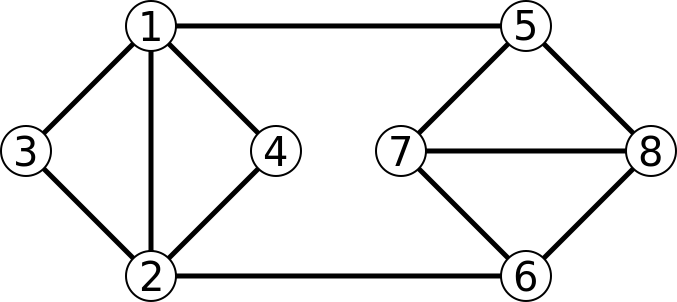
\includegraphics[width=0.5\textwidth]{JKMP_graphe.png}
    \caption{Représentation du plus petit graphe où DSATUR n'est pas optimal (8 sommets, 12 arêtes).}
    \label{fig:dsatur_non_optimal_graph}
\end{figure}
\paragraph{Coloration obtenue par DSATUR sur le graphe de la figure 1:} \\
\begin{itemize}
    \item \textbf{Rouge} : Sommets 1, 7
    \item \textbf{Vert} : Sommets 3, 4, 8
    \item \textbf{Bleu} : Sommets 2, 5
    \item \textbf{Jaune} : Sommet 6
\end{itemize}

\paragraph{Coloration optimale sur le graphe de la figure 1 :} \\
\begin{itemize}
    \item \textbf{Rouge} : Sommets 1, 7
    \item \textbf{Vert} : Sommets 3, 4, 5, 6
    \item \textbf{Bleu} : Sommets 2, 8
\end{itemize}

---

\subsection{Objectifs spécifiques de notre projet}

Ce projet vise à mettre en œuvre l'algorithme DSATUR en utilisant le langage OCaml. Les objectifs spécifiques sont les suivants :
\begin{itemize}
    \item \textbf{Implémentation} : développer une version fonctionnelle et robuste de DSATUR en exploitant les structures de données et les fonctionnalités offertes par OCaml.
    \item \textbf{Analyse des performances} : évaluer l'efficacité de l'algorithme sur des graphes de tailles et de structures variées.
    \item \textbf{Défis techniques} : identifier les limitations éventuelles de l'implémentation et proposer des améliorations ou des solutions alternatives.
\end{itemize} 

---

\section{Méthodes et implémentation}

\subsection{Organisation du travail}

Le projet a suivi une approche itérative avec plusieurs phases de développement et d'expérimentation. Voici les étapes principales :
\begin{itemize}
    \item \textbf{Phase initiale} : mise en œuvre d’une structure simple pour les graphes sous forme de tableau de listes adjacentes. Les premières versions utilisaient des parcours exhaustifs et des fonctions basiques pour sélectionner les sommets à colorier.
    \item \textbf{Amélioration des critères de sélection} : intégration des calculs de DSAT (Degree of Saturation) pour prioriser les sommets avec des saturations maximales. Cette version s’appuyait sur des tableaux pour stocker dynamiquement les saturations des sommets.
    \item \textbf{Introduction du tas binaire} : afin d’optimiser la sélection des sommets, un tas binaire a été intégré dans la version finale. Cette structure a permis une gestion efficace des priorités et une amélioration significative des performances.
\end{itemize}
Cette approche itérative a permis de valider chaque étape et d’améliorer progressivement les performances de l’algorithme.


---

\subsection{Structures de données et algorithmes}

Pour résoudre efficacement le problème de la coloration de graphes avec DSATUR, plusieurs choix techniques ont été faits :
\begin{itemize}
    \item \textbf{Représentation des graphes} : un graphe \( G = (S, A) \) est représenté comme un tableau de listes adjacentes. Chaque sommet \( s \in S \) est associé à une liste contenant ses voisins. Cette structure permet un accès rapide aux sommets adjacents, essentiel pour le calcul du DSAT.
\end{itemize}

\noindent Voici un exemple de représentation d’un graphe simple avec 4 sommets (\( S = \{0, 1, 2, 3\} \)) et 5 arêtes (\( A = \{ \{0, 1\}, \{0, 2\}, \{1, 2\}, \{1, 3\}, \{2, 3\} \} \)) :
\begin{center}
    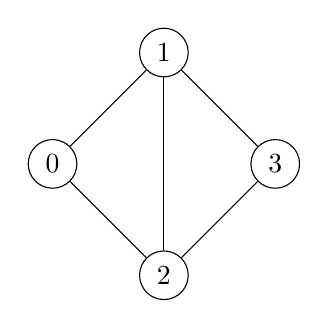
\begin{tikzpicture}[node distance=2cm and 2cm]
        % Les sommets
        \node (0) [circle, draw] {0};
        \node (1) [circle, draw, above right of=0] {1};
        \node (2) [circle, draw, below right of=0] {2};
        \node (3) [circle, draw, below right of=1] {3};

        % Les arêtes
        \draw (0) -- (1);
        \draw (0) -- (2);
        \draw (1) -- (2);
        \draw (1) -- (3);
        \draw (2) -- (3);
    \end{tikzpicture}
\end{center}
\[
\text{Tableau de listes adjacentes} :  
\begin{array}{|c|c|}
\hline
\text{Sommet} & \text{Voisins} \\
\hline
0 & [1, 2] \\
1 & [0, 2, 3] \\
2 & [0, 1, 3] \\
3 & [1, 2] \\
\hline
\end{array}
\]

\begin{itemize}
    \item \textbf{Gestion des priorités} : un \textbf{tas binaire} a été intégré pour gérer dynamiquement les sommets en fonction de leur DSAT (\textit{Degree of Saturation}). Cette structure garantit que le sommet ayant le DSAT le plus élevé est toujours traité en priorité. En cas d'égalité de DSAT entre plusieurs sommets, le choix est fait en fonction de leur degré. L’utilisation d’un tas réduit la complexité de la sélection des sommets à \( O(\log n) \), améliorant significativement les performances par rapport à un tri linéaire.
    \item \textbf{Calcul dynamique du DSAT} : à chaque itération, le DSAT d’un sommet est mis à jour pour refléter les couleurs attribuées à ses voisins. Cette opération est réalisée en temps linéaire par rapport au degré du sommet concerné, garantissant une mise à jour rapide même pour des graphes denses.
\end{itemize}

---

\subsection{Implémentation en OCaml}

Le langage OCaml a été imposé comme cadre de développement pour ce projet. OCaml s'est avéré adapté pour aborder les défis spécifiques liés à la mise en œuvre de l'algorithme DSATUR adaptés à la programmation fonctionnelle. Voici quelques observations concernant ses caractéristiques :

\begin{itemize}
    \item \textbf{Rigueur et sûreté} : OCaml, avec son typage statique, aide à réduire les erreurs lors du développement, en particulier pour les algorithmes complexes impliquant de nombreuses structures de données.
    \item \textbf{Gestion fonctionnelle des données} : sa nature fonctionnelle favorise une approche déclarative et facilite la manipulation des structures immuables
\end{itemize}

---

\section{Évolution et gestion du projet}

Le développement du projet a suivi une méthodologie itérative, avec des validations successives pour garantir une implémentation fiable et performante. Cette approche a permis de surmonter plusieurs défis techniques et d'améliorer progressivement l'algorithme.

---

\subsection{Première phase : Mise en place des bases}

La première étape du projet a consisté à représenter les graphes sous forme de tableaux de listes adjacentes. Cette représentation, bien adaptée aux opérations fréquentes comme la recherche des voisins, a servi de fondation pour les implémentations ultérieures.

Dans cette phase, les sommets étaient sélectionnés de manière exhaustive, à l'aide d'une boucle parcourant tous les sommets pour identifier celui ayant le DSAT et le degré les plus élevés. Bien que cette approche ait permis de valider le fonctionnement initial de l'algorithme, ses performances étaient limitées pour des graphes de taille importante (\( O(n^2) \)).

---

\subsection{Deuxième phase : Optimisation du calcul de DSAT}

Pour réduire la complexité, une version améliorée a introduit un tableau de stockage des valeurs de DSAT. Ce tableau était mis à jour dynamiquement après chaque étape de coloration. Cette optimisation a eu un impact significatif sur les performances en éliminant le recalcul systématique des saturations, rendant ainsi le programme beaucoup plus efficace pour des graphes de taille moyenne.

Un défi rencontré dans cette phase concernait la gestion des mises à jour dynamiques. Il a été nécessaire de bien gérer les références mutables dans OCaml pour éviter les erreurs dans les mises à jour simultanées des sommets et de leurs voisins.

---

\subsection{Troisième phase : Introduction d’un tas binaire}
\subsubsection{Arbres tournois} 
Un \textit{arbre tournoi} est un arbre binaire étiqueté par des éléments d’un ensemble totalement ordonné $(K, \leq)$, tel que pour tout nœud, l'étiquette de ce nœud est supérieure à celles de tous ses descendants.\cite{data_structure_complements}

Les arbres tournois permettent des opérations efficaces, telles que :
\begin{itemize}
    \item \textbf{Extraction du maximum} : $\mathcal{O}(h)$, en fusionnant les sous-arbres ou par \textit{percolation descendante}.
    \item \textbf{Insertion} : $\mathcal{O}(h)$, par \textit{percolation ascendante}.
    \item \textbf{Modification de priorité} : $\mathcal{O}(h)$.
\end{itemize}

Ces propriétés les rendent adaptés pour des applications nécessitant un accès rapide au maximum ou des modifications dynamiques.

\vspace{0.5cm}

---

\subsubsection{Tas binaires}
Un \textit{tas binaire} est un arbre parfait qui respecte une propriété d’ordre : \cite {data_structure_complements}
\begin{itemize}
    \item \textbf{Tas max} : La valeur de chaque nœud est supérieure ou égale à celles de ses descendants.
    \item \textbf{Tas min} : La valeur de chaque nœud est inférieure ou égale à celles de ses descendants.
\end{itemize}

Les tas binaires sont souvent représentés sous forme de tableaux pour une gestion efficace :
\begin{itemize}
    \item La racine est à l'indice $0$.
    \item Les fils gauche et droit d’un nœud à l’indice $i$ sont aux indices $2i+1$ et $2i+2$.
    \item Le parent d’un nœud à l’indice $i$ est à l’indice $\lfloor \frac{i-1}{2} \rfloor$.
\end{itemize}

Cette représentation permet des opérations optimisées, telles que l'ajout, la suppression ou la réorganisation, en temps logarithmique $\mathcal{O}(\log n)$.

---

\subsubsection{Intégration dans notre projet}


La version finale a intégré un tas binaire pour optimiser la gestion des priorités. En remplaçant la recherche linéaire par une gestion hiérarchisée des sommets en fonction de leur DSAT et de leur degré, cette structure a réduit la complexité de sélection à \( O(\log n) \).

Avant cette amélioration, l’algorithme stagnait sur des graphes de taille modeste, avec un maximum d’environ 60 sommets, en raison des limitations de performances dues à la recherche linéaire des sommets. L’introduction du tas binaire a permis de traiter efficacement des graphes de plusieurs centaines de sommets, rendant l’algorithme plus performant.


L'intégration du tas binaire a toutefois introduit de nouveaux défis :
\begin{itemize}
    \item Mise à jour des priorités : chaque fois qu’un sommet était coloré, il fallait réorganiser le tas pour refléter les nouvelles saturations des sommets voisins.
    \item Gestion des champs mutables : des erreurs pouvaient survenir si les champs des sommets n’étaient pas correctement synchronisés avec leur position dans le tas.
\end{itemize}

Ces problèmes ont été résolus en testant intensivement chaque fonction manipulant le tas et en vérifiant systématiquement la cohérence des données sur des graphes de petite taille.

En parallèle, une version utilisant un algorithme de \textit{Branch and Bound} a été développée pour garantir l'optimalité. Bien que cette méthode fournisse le nombre chromatique exact, elle s’est avérée trop lente en pratique : le temps de calcul devenait prohibitif pour des graphes comportant plus de 40 sommets. Cette limitation est inhérente à la nature exhaustive du Branch and Bound, qui explore toutes les combinaisons possibles pour trouver la solution optimale.

---

\subsection{Validation et tests}

Chaque étape de développement a été accompagnée de tests sur des graphes issus de la bibliothèque DIMACS ainsi que sur des graphes simples créés manuellement. Ces tests ont permis de :
\begin{itemize}
    \item Vérifier la robustesse de l’algorithme face à des cas limites .
    \item Comparer les résultats obtenus avec les nombres chromatiques connus pour certains graphes.
\end{itemize}

Les résultats obtenus ont confirmé les améliorations successives et ont validé la pertinence des choix techniques.

---

\subsection{Bilan des améliorations}

En passant d’une approche naïve à une version optimisée avec un tas binaire, le projet a permis de :
\begin{itemize}
    \item Réduire significativement le temps d’exécution pour des graphes de grande taille.
    \item Garantir une allocation optimale des couleurs avec un algorithme robuste et fiable.
    \item Mettre en lumière l’importance d’une gestion efficace des priorités et des structures de données adaptées.
\end{itemize}

Ces évolutions successives témoignent de l’importance d’une approche itérative dans le développement d’algorithmes complexes, et des bénéfices d’un processus d’évaluation et de validation continue.

\section{Résultats et analyse}

\subsection{Méthodologie des tests}

Pour évaluer les performances de l’algorithme DSATUR, nous avons utilisé des graphes issus de la bibliothèque \href{https://mat.tepper.cmu.edu/COLOR/instances.html}{DIMACS Graph Instances}, ainsi que des graphes simples créés manuellement pour valider le bon fonctionnement de l’implémentation. 

Les critères d’évaluation incluent :
\begin{itemize}
    \item Le \textbf{nombre chromatique} obtenu par l’algorithme, comparé aux nombres chromatiques connus pour certains graphes.
    \item Le \textbf{temps d’exécution} mesuré pour des graphes de tailles et de structures variées.
    \item La \textbf{robustesse de l’algorithme} face à des cas limites, tels que des graphes fortement connectés, des graphes bipartis, ou des graphes clairsemés.
\end{itemize}

Les tests ont été réalisés sur une machine standard. Il est important de noter que les performances des algorithmes peuvent varier en fonction de l'architecture matérielle utilisée (processeur, mémoire vive, etc.). Les résultats présentés ici sont donc indicatifs et peuvent différer selon les environnements d'exécution.
 Les résultats présentés reflètent l’impact des différentes optimisations intégrées au cours du projet, notamment l’ajout du tas binaire.

---

\subsection{Présentation des résultats}

Les résultats obtenus sont résumés dans le tableau suivant :

\begin{table}[h!]
    \centering
    \resizebox{\textwidth}{!}{
    \begin{tabular}{|c|c|c|c|c|c|}
        \hline
        \textbf{Graphe} & \textbf{Sommets} & \textbf{Arêtes} & \textbf{Nombre chromatique attendu} & \textbf{Nombre chromatique obtenu} & \textbf{Temps (s)} \\
        \hline
        myciel3 & 11 & 20 & 4 & 4 & 0.000213 \\
        \hline
        myciel6 & 95 & 755 & 7 & 7 & 0.004122 \\
        \hline
        mulsol.i.4 & 307 & 3925 & 31 & 31 & 0.051327 \\
        \hline
        miles1500 & 128 & 6454 & 73 & 73 & 0.120378 \\
        \hline
        homer & 561 & 3253 & 13 & 13 & 0.025140 \\
        \hline
        school1 & 385 & 19095 & 17 & 17 & 0.354306 \\
        \hline
        queen8\_12 & 96 & 1368 & 12 & 14 & 0.011529 \\
        \hline
    \end{tabular}
    }
    \caption{Résultats des tests sur différents graphes}
    \label{tab:results}
\end{table}

Les graphes issus de la bibliothèque DIMACS (comme \textit{myciel} et \textit{queen}) ont permis de tester la capacité de l’algorithme à traiter des graphes connus, tandis que des graphes générés manuellement ont servi à explorer des configurations spécifiques.

Sur l’ensemble des graphes DIMACS testés, l’algorithme DSATUR a régulièrement trouvé le \textbf{nombre chromatique optimal}, validant ainsi son efficacité sur des instances bien définies.

---

\subsection{Analyse des performances}

Les résultats montrent que :
\begin{itemize}
    \item Pour des graphes de taille modeste (ex. \textit{myciel3}, \textit{myciel4}), l’algorithme obtient systématiquement le nombre chromatique optimal.
    \item L’introduction du tas binaire a permis de \textbf{réduire significativement les temps d’exécution}, en particulier pour des graphes comportant plusieurs centaines de sommets.
    \item Les graphes fortement connectés (avec de nombreuses arêtes par rapport au nombre de sommets) nécessitent davantage de couleurs et augmentent légèrement le temps de calcul.
    \item Les graphes bipartis et les graphes clairsemés sont résolus rapidement grâce à leur structure particulière, qui limite les contraintes sur les couleurs.
\end{itemize}

Cependant, pour des graphes très denses ou des structures complexes comme \textit{Mycielski}, l’algorithme DSATUR peut échouer à atteindre l’optimalité dans certains cas, bien que les résultats soient souvent proches du nombre chromatique réel.

Une version utilisant l’algorithme \textit{Branch and Bound} a également été implémentée pour vérifier l'optimalité des solutions. Toutefois, cette approche, malgré sa précision, s’est révélée impraticable pour des graphes dépassant 40 sommets, en raison de sa complexité exponentielle.

---

\subsection{Impact des optimisations}

Les optimisations successives ont eu un impact significatif sur les performances globales de l’algorithme :
\begin{itemize}
    \item La gestion des priorités avec un \textbf{tas binaire} a permis de réduire la complexité de sélection des sommets de \( O(n) \) à \( O(\log n) \), rendant l’algorithme scalable pour des graphes de plusieurs centaines de sommets.
    \item Le \textbf{calcul dynamique du DSAT}, combiné à une mise à jour efficace des priorités, a éliminé le recalcul exhaustif des saturations, améliorant ainsi les temps de traitement pour des graphes de taille moyenne.
\end{itemize}

Ces résultats confirment l’efficacité des choix techniques et mettent en lumière l’importance des structures de données adaptées dans le contexte de la coloration de graphes.

---

\section{Bonus : Coloration de Graphes avec Réduction SAT}

Pour compléter l'algorithme DSATUR, nous avons exploré une méthode alternative basée sur la réduction du problème de \(k\)-coloration en une instance SAT. Cette approche tire parti des solveurs SAT pour trouver une coloration valide d'un graphe donné.
Dans ces fichiers \cite{k_coloring_sat} \cite{coloring_course}, une méthode est proposée pour transformer un problème de \(k\)-coloration en une instance SAT, permettant de tirer parti de solveurs SAT pour garantir une solution optimale.

Un point notable de cette partie est la réutilisation et l'adaptation d'un SAT solver basique développé lors de l'un de mes projets en classe préparatoire \cite{duff_sat_solver}.

---

\subsection{Principe de la Réduction SAT}

Dans cette méthode, chaque sommet \(i \in S\) est associé à \(k\) variables propositionnelles \(v_{i,k}\), où \(v_{i,k}\) signifie que le sommet \(i\) est coloré avec la couleur \(k\). Pour garantir une \(k\)-coloration valide, les contraintes suivantes sont imposées :

\begin{itemize}
    \item \textbf{Chaque sommet a exactement une couleur :}
        \begin{itemize}
            \item \textit{Au moins une couleur :} Chaque sommet \(i \in S\) doit avoir au moins une couleur. Cette contrainte est exprimée par la clause suivante :
            \[
            \forall i \in S : (v_{i,1} \lor v_{i,2} \lor \ldots \lor v_{i,k})
            \]
            \item \textit{Au plus une couleur :} Un sommet \(i \in S\) ne peut pas avoir plus d'une couleur. Cette contrainte est exprimée par :
            \[
            \forall i \in S, \forall 1 \leq r < q \leq k : (\neg v_{i,r} \lor \neg v_{i,q})
            \]
        \end{itemize}
    \item \textbf{Pas de conflit entre sommets adjacents :} Deux sommets adjacents \(i, j \in S\) (avec \((i, j) \in A\)) ne peuvent pas avoir la même couleur. Cette contrainte est exprimée par :
    \[
    \forall k \in \{1, \ldots, k\}, \forall (i, j) \in A : (\neg v_{i,k} \lor \neg v_{j,k})
    \]
\end{itemize}

Ces contraintes sont combinées pour construire une formule en forme normale conjonctive (CNF), qui est ensuite résolue à l'aide d'un solveur SAT.

---

\subsection{Implémentation}

Notre implémentation suit ces étapes :
\begin{enumerate}
    \item \textbf{Lecture du Graphe :} Les graphes sont lus au format DIMACS (\texttt{.col}), avec extraction des sommets et des arêtes.
    \item \textbf{Génération des Clauses CNF :} Les contraintes ci-dessus sont traduites en clauses, en assignant une variable unique à chaque paire sommet/couleur.
    \item \textbf{Résolution :} Les formules CNF générées sont résolues à l'aide des algorithmes Quine et DPLL.
    \item \textbf{Recherche du Plus Petit \(k\) :} Un processus itératif ajuste \(k\) pour trouver le plus petit nombre de couleurs nécessaires.
\end{enumerate}

---

\subsection{Résultats et Analyse}

La méthode a été testée sur plusieurs graphes issus de la bibliothèque DIMACS, tels que \texttt{myciel3.col} et \texttt{queen5\_5.col}. Les résultats montrent que la réduction SAT fournit des solutions optimales pour des graphes de taille modérée.

\begin{table}[h!]
\centering
\begin{tabular}{|c|c|c|c|c|}
\hline
\textbf{Graphe} & \textbf{Sommets} & \textbf{Arêtes} & \textbf{\(k\) trouvé} & \textbf{Temps (s)} \\ \hline
\texttt{myciel3.col} & 11 & 20 & 4 & 0.012623 \\
\texttt{queen5\_5.col} & 25 & 160 & 5 & 0.605836 \\
\texttt{queen6\_6.col} & 36 & 290 & 7 & 413.921886 \\
\hline
\end{tabular}
\caption{Résultats obtenus avec la méthode SAT}
\label{tab:sat_results}
\end{table}
\paragraph{Remarque :} Pour le graphe \texttt{queen6\_6.col}, la formule CNF correspondante contient \textbf{252 variables} et \textbf{4852 clauses}.

---

\subsection{Avantages et Limites}

L'approche basée sur la réduction SAT présente les avantages suivants :
\begin{itemize}
    \item Garantie de trouver une solution optimale pour un \(k\) donné.
    \item Applicabilité à une large variété de graphes.
\end{itemize}

Cependant, cette méthode est limitée par :
\begin{itemize}
    \item La taille exponentielle de la formule CNF générée, qui rend la méthode impraticable pour des graphes de grande taille.
    \item Le temps de résolution des formules CNF, qui augmente rapidement avec \(k\) et la densité du graphe.
\end{itemize}
---
\subsection{Perspectives}

Pour améliorer cette méthode, il serait intéressant d'intégrer des solveurs SAT externes, tels que \texttt{MiniSat} ou \texttt{Glucose}, qui sont optimisés pour des formules de grande taille. De plus, des techniques de prétraitement, comme la simplification des graphes ou l'utilisation de heuristiques pour initialiser \(k\), pourraient réduire significativement la complexité.

---
\section{Comparaison des Approches : DSATUR et Réduction SAT}

Dans cette section, nous comparons les deux méthodes implémentées pour résoudre le problème de coloration de graphes : l'approche heuristique basée sur l'algorithme DSATUR et l'approche exacte utilisant la réduction SAT. Ces deux méthodes offrent des perspectives complémentaires en termes de performances et de précision.

---

\subsection{Critères de Comparaison}

Pour évaluer les deux approches, nous nous basons sur les critères suivants :
\begin{itemize}
    \item \textbf{Temps d'exécution} : Mesuré sur des graphes de tailles et de densités variées.
    \item \textbf{Optimalité des solutions} : Qualité de la solution trouvée, comparée au nombre chromatique réel (lorsqu'il est connu).
    \item \textbf{Scalabilité} : Capacité à gérer des graphes plus grands ou plus complexes.
    \item \textbf{Facilité d'implémentation} : Complexité des algorithmes et des structures de données utilisées.
\end{itemize}

---

\subsection{Avantages et Inconvénients des Approches}

\subsubsection{Algorithme DSATUR}

L'algorithme DSATUR est une méthode heuristique qui se base sur le degré de saturation des sommets pour guider la coloration.

\paragraph{Avantages :}
\begin{itemize}
    \item \textbf{Rapidité} : DSATUR est rapide et efficace pour des graphes de tailles modérées.
    \item \textbf{Implémentation simple} : Les structures de données utilisées (listes d'adjacence, tableaux) sont simples et bien adaptées.
    \item \textbf{Solutions proches de l'optimalité} : Dans de nombreux cas, DSATUR produit une solution avec un nombre de couleurs proche du nombre chromatique.
\end{itemize}

\paragraph{Inconvénients :}
\begin{itemize}
    \item \textbf{Résultats non garantis} : DSATUR ne garantit pas une solution optimale.
    \item \textbf{Sensibilité à l'ordre des sommets} : Les résultats peuvent varier en fonction de l'ordre initial des sommets.
\end{itemize}

---

\subsubsection{Réduction SAT}

L'approche par réduction SAT est une méthode exacte qui traduit le problème en une formule CNF résolue à l'aide d'un solveur SAT (Quine/DPLL).

\paragraph{Avantages :}
\begin{itemize}
    \item \textbf{Optimalité garantie} : Si une solution existe pour un \(k\) donné, la méthode la trouvera.
    \item \textbf{Flexibilité} : Permet de résoudre des variantes du problème de coloration en modifiant les contraintes CNF.
\end{itemize}

\paragraph{Inconvénients :}
\begin{itemize}
    \item \textbf{Coût computationnel élevé} : La taille des formules CNF et le temps de résolution augmentent rapidement avec la taille du graphe.
    \item \textbf{Complexité d'implémentation} : La construction des formules CNF et l'optimisation du solveur nécessitent des efforts supplémentaires.
\end{itemize}

---

\subsection{Comparaison des Performances}

Les deux approches ont été testées sur des graphes issus de la bibliothèque DIMACS, avec des résultats résumés dans le tableau~\ref{tab:comparaison}.

\begin{table}[h!]
\centering
\begin{tabular}{|c|c|c|c|c|c|}
\hline
\textbf{Méthode} & \textbf{Graphe} & \textbf{Sommets} & \textbf{Arêtes} & \textbf{\(k\) trouvé} & \textbf{Temps (s)} \\ \hline
DSATUR & \texttt{myciel3.col} & 11 & 20 & 4 & 0.000213 \\
SAT & \texttt{myciel3.col} & 11 & 20 & 4 & 0.012623 \\ \hline
DSATUR & \texttt{queen5\_5.col} & 25 & 160 & 5 & 0.001922 \\
SAT & \texttt{queen5\_5.col} & 25 & 160 & 5 & 0.605836 \\ \hline
DSATUR & \texttt{queen6\_6.col} & 36 & 290 & 9 & 0.003249 \\
SAT & \texttt{queen6\_6.col} & 36 & 290 & 7 & 413.921886 \\ \hline
\end{tabular}
\caption{Comparaison des performances de DSATUR et SAT}
\label{tab:comparaison}
\end{table}

Les résultats montrent que :
\begin{itemize}
    \item DSATUR est mieux adapté pour des graphes de grande taille ou lorsque le temps de calcul est critique.
    \item La réduction SAT, bien que coûteuse en temps de calcul, garantit des solutions optimales et peut être utilisée pour valider les résultats heuristiques.
\end{itemize}

En pratique, une approche hybride pourrait être envisagée : utiliser DSATUR pour obtenir une solution initiale, puis vérifier ou affiner cette solution à l'aide de la méthode SAT.

---

\section{Conclusion et Perspectives}

Dans ce rapport, nous avons étudié le problème de la coloration de graphes, en mettant en œuvre deux approches distinctes : l'algorithme DSATUR, une méthode heuristique, et une approche exacte basée sur la réduction SAT. Ces deux méthodes offrent des perspectives complémentaires, chacune étant adaptée à des cas d'utilisation spécifiques.

L'algorithme DSATUR a démontré son efficacité en fournissant rapidement des solutions proches de l'optimalité pour des graphes de taille modérée. Cependant, il ne garantit pas une solution optimale, ce qui peut être une limitation pour certaines applications nécessitant une rigueur absolue.

En revanche, la réduction SAT, bien que coûteuse en termes de temps de calcul et de mémoire, offre une garantie d'optimalité. Elle se distingue également par sa flexibilité, permettant d'adresser des variantes complexes du problème de coloration. Les tests réalisés montrent que cette méthode est adaptée à des graphes de taille modérée, mais elle devient impraticable pour des graphes très grands ou très denses.

---

\subsection{Perspectives}

Pour aller plus loin, plusieurs pistes d'amélioration peuvent être envisagées :
\begin{itemize}
    \item \textbf{Optimisation de DSATUR} : Intégration de structures de données avancées, comme des tas binaires ou des tableaux de priorités, pour améliorer les performances sur des graphes de grande taille.
    \item \textbf{Utilisation de solveurs SAT externes} : Intégrer des outils performants comme \texttt{MiniSat} ou \texttt{Glucose} \cite{sat_glucose} , capables de gérer des formules CNF de grande taille.
    \item \textbf{Approches hybrides} : Combiner DSATUR et SAT pour exploiter leurs avantages respectifs. Par exemple, utiliser DSATUR pour trouver une solution initiale, puis vérifier ou affiner cette solution avec un solveur SAT.
    \item \textbf{Exploration de variantes du problème} : Étendre les implémentations pour résoudre des variantes telles que la coloration d'arêtes, la coloration pondérée ou les graphes dynamiques.
    \item \textbf{Applications concrètes} : Tester les algorithmes sur des cas réels, comme la planification d'emplois du temps, l'affectation de fréquences radio, ou l'optimisation de ressources dans les réseaux.
\end{itemize}

Ce projet a permis d'explorer des approches complémentaires pour résoudre un problème classique en théorie des graphes, tout en offrant une base solide pour des recherches futures dans ce domaine.

\begin{thebibliography}{99}

\bibitem{dsatur_wikipedia}
Wikipedia. (2023). \textit{DSatur}. Disponible sur : \url{https://en.wikipedia.org/wiki/DSatur}.

\bibitem{brelaz1979}
Brélaz, D. (1979). \textit{New methods to color the vertices of a graph}. Communications of the ACM, 22(4), 251–256.
\\ URL: \url{https://dl.acm.org/doi/10.1145/359094.359101}

\bibitem{dimacs1993}
Johnson, D. S., \& Trick, M. A. (1993). \textit{DIMACS Graph Coloring Benchmark Instances}. DIMACS Series in Discrete Mathematics and Theoretical Computer Science. 
\\ URL: \url{https://mat.tepper.cmu.edu/COLOR/instances.html}

\bibitem{graph_theory_course}
Rouhling D. rédigé par Lasercata (2021 MP2I Lycée Victor Hugo). \textit{Cours de théorie des graphes}. Disponible sur GitHub : \url{https://github.com/lasercata/MP2I/blob/main/1.MP2I/0.Info/Chap_10__Graph_theory/Info_chap_10__Graph_theory.pdf}.

\bibitem{data_structure_complements}
Rouhling D. rédigé par Lasercata (2021 MP2I Lycée Victor Hugo). \textit{Cours de complément sur les structures de données}. Disponible sur GitHub : \url{https://github.com/lasercata/MP2I/blob/main/1.MP2I/0.Info/Chap_06__Data_structure_complements/Info_chap_6__Data_structure_complements.pdf}.

\bibitem{greedy_algorithms}
Robert, Y. (2023). \textit{Cours d'algorithmes gloutons}. ENS Lyon. Disponible sur : \url{https://graal.ens-lyon.fr/~yrobert/algoL3/3-greedy.pdf}.

\bibitem{smallest_hard_dsatur}
J.~Kratochvíl, Z.~Tuza, M.~Voigt (2001). \textit{The smallest hard-to-color graph for algorithm DSAT}. Discrete Mathematics, 233, 255–261.  
URL: \url{https://www.sciencedirect.com/science/article/pii/S0012365X00004398}

\bibitem{k_coloring_sat}
Antonin Novak. (2022). \textit{Solving the Graph \(k\)-Coloring Problem using SAT Reduction}. Disponible sur : \url{https://cw.fel.cvut.cz/b212/_media/courses/rm35koa/k_coloring_sat.pdf}.

\bibitem{coloring_course}
Lifschitz, V. (2006). \textit{Notes on Graph Coloring}. Disponible sur : \url{https://www.cs.utexas.edu/~vl/teaching/lbai/coloring.pdf}.

\bibitem{duff_sat_solver}
Dufrenois, M. (2023). \textit{SatSolver}. Dépôt GitHub. Disponible sur : \url{https://github.com/DUFF13/SatSolver}.

\bibitem{sat_glucose}
Audemard, G., \& Simon, L. (2009). \textit{Glucose: A solver for SAT problems}. International Journal on Artificial Intelligence Tools, 27(1), 107-128.
\\ URL: \url{https://www.labri.fr/perso/lsimon/glucose/}

\end{thebibliography}



\end{document}
